Am nähesten zu der \textbf{PAC}\footnote{Port-Adapter-Controller} Struktrur 
ist das Pattern \textbf{MVP} (siehe Kapitel \ref{kap:MVP}).
Dabei entsprechen die Aufgaben von \textbf{View} (Benutzerobefläche aktualisieren und Ereignisse empfangen) den Aufgaben von \textbf{Port}. 
Die Aufgaben von \textbf{Presenter} (Ereignisse von der Benutzerobefläche in das Datenmodel der Anwendung umwandlen) entsprechen den Aufgaben \textbf{Adapter}.
Und die Aufgaben von dem Rest des Programms inklusiv \textbf{Controller} entspechen den Aufgaben von \textbf{Model} (ankommende Ereignisse abarbeiten und das Ergebnis zurückgeben).

Der Unterschied zu \textbf{MVP} besteht darin, dass \textbf{MVP} im klassischen Sinne nur für die Benutzerobeflächen gedacht ist,
während es in der hier beschriebenen Umsetzung für alle Schnittstellen benutzt wird.
\textbf{MVP} Architektur übernimmt in der gesamten Application eine zentralle Stelle und ist nur einmal vorhanden.
\textbf{PAC} ist nur ein Teil der gesamten Application, wird an mehreren Stellen unterschiedlich benutzt und beschreibt nicht 
die komplette Architektur der Application.

Die Aufgabe von jeder \textbf{PAC}-Struktur ist die Steurung von einem Aufgabengebiet (z.B. HTTP Schnittstelle oder OCPP Schnittstelle).
Der Grund für das Aufteilen in 3 verschiedene Teile (Adapter, Port und Controller) ist
\textbf{SRP} (Kapitel \ref{kap:SRP}). Somit hat jeder Teil eine Aufgabe und lässt sich besser im Laufe der Zeit
warten. 


\begin{figure}[H]
   \centering
   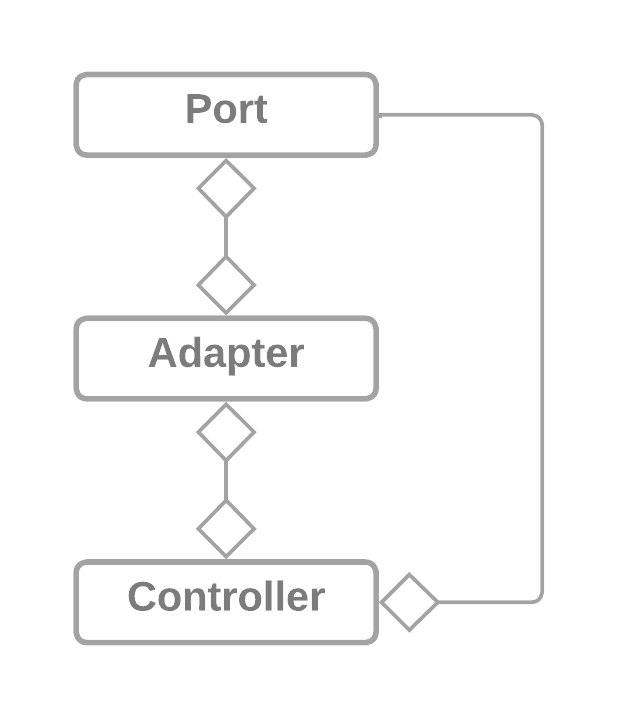
\includegraphics[width=5.5cm]{./images/Port-Adapter-Contoller.png}
    \caption[Objektendiagramm PAC]{Objektendiagramm PAC}
    \label{fig:CDPAC}
\end{figure}